%%%% This is the general thesis/project report template for most users
\documentclass[showtrims]{rubook}
%% RU Book options (subclass of memoir)
%% a4paper or b5paper(default):  paper stock size.
%%     If A4, show cut lines.  If b5, no cut lines.
\usepackage[]{ruthesis}
%% Options for ruthesis in []:
%%   IS Icelandic is main language, otherwise default to English

%%%%%% Packages and Macros %%%%%%%%%%%%%%%%%%%%%%%%%%%%%%%%
\usepackage{custom}
%% Commonly-used packages and macros are in custom.sty
%% Put any additional packages after this line
%% !!WARNING: The geometry package is incompatible with this template!


\graphicspath{{graphics/}{Graphics/}{./}}
%% This is a list of folders to search for graphics files to include
%% for the graphicx package (already loaded).  This may be case-sensitive.
%% LaTeX will search from left to right in the list, so you can put "cropped" versions
%% in the first directory and it will grab them first. e.g.
%\graphicspath{{graphics-cropped/}{graphics/}{Graphics/}{./}}

%%%%%%%%%%%%%%%%%%%%%%%%%%%%%%%%%%%%%%%%%%%%%%%%%%%%%%%

\title{Reducing wheelchair dependency with a semi-autonomous following wheelchair}
\author{Klara~Kristmundsdóttir\\Margrét~Eiríksdóttir\\Sævar~Örn~Valsson \\Þórfríður~Ina~Arinbjarnardóttir}
\date{2023}{2}{16}%{Year}{Month}{Day}%use numbers

%\DocumentInfo{TYPE}{ABBREVIATION}{DEGREE}{PROGRAM}{ECTS}{School/Department}
\DocumentInfo{Thesis}{M.Sc.}{Master of Science}{Mechatronics}{30}{Department of Engineering}
\DocumentDescription{T620-ENGX EngineeringX Project Report for Team 17, Section CLINX}
% Change this if you need a custom title or if it needs to be in Icelandic

%% PhD only have Thesis Committee with roles.  Examiner is part of committee.
\SupervisorHeading{EngineeringX Evaluators}
\Supervisors{
  \personinfo{Joseph T. Foley}{Head Instructor}{Professor}{Reykjavík University}{Iceland}
  \personinfo{Paolo Gargiulo}{Section Instructor}{Professor}{Reykjavík University}{Iceland}
  \personinfo{Arnar Evgení Gunnarsson}{Section TA}{Student}{Reykjavík University}{Iceland}
  \personinfo{Jón Stefánsson} {Stakeholder}{Student}{Reykjavík University}{Iceland}
  \personinfo{Kári Halldórsson} {Stakeholder}{Professor}{Reykjavík University}{Iceland}
}

\begin{document}
%% TODO: get the official cover graphic and have the system fill in the fields for you
\maketitle{}
\copyrightpage{}
% If this is a PhD, register for an ISSN and ISBN, then:
% \copyrightpage{ISSN xxxx-yyyy\\ISBN 978-xxxxxxxxxx\\\url{http://hdl.handle.net/1946/xxxx}\\}
%\signaturepage{} %Generally only for Print copies

%\begin{dedications}% Optional
%  I dedicate this to my spouse/child/pet/power animal.
%\end{dedications}

\enableindents{}% turn on/off paragraph indents
% RUM: "Acknowledgements (optional)"%start numbering

\clearpage{}
\tableofcontents{}\clearpage
\listoffigures{}\clearpage
\listoftables{}\clearpage

%% A list of abbreviations is an example of a special list
%% Other lists may be added, such as lists of algorithms, symbols, theorems, etc.
%% IN CS PhD, this is sometimes centered.
\chapter*{List of Abbreviations}%%RUM: Not mentioned
%% This list demonstrates the "siunitx" package capabilities
\begin{tabular}{ll}
Abbreviation &Description \\
N/A & Not Applicable \\ %New function:  \unit{} in Livetex 2021
N/S & Not Specified \\ %New function:  \unit{} in Livetex 2021 
\end{tabular}
\begin{abstract}
    Our project is an semi-autonomous following wheelchair for wheelchair users that are not bound to the chair and want to enhance their ability to walk to reduce the use of the wheelchair.
    
    \newline
    \url{https://www.overleaf.com/project/63eb75216632895377abdad8}

  %The goal of this template is to produce electronic output to be uploaded to Skemman that can be later printed out and bound into a professional looking textbook that fits on standard library shelves.
  %It is important to note that A4 paper when bound requires taller shelf spacing, so the B5 paper format was chosen instead.
  %When binding a book, the edges that face outward need to be very smooth to reduce contamination and dust from entering the book when it sits on a shelf; this is why traditionally a larger paper size is cut down to the book size.
  %If your print house expects the stock to be A4, then make sure the rubook has the ``a4paper'' option.
  %If they prefer to deal with preparation themselves from a B5 pdf, then the default ``b5paper'' option is correct.
  %The template is optimized for lualatex, but should still work with pdflatex.
  
  %The abstract goes here in English or Icelandic.
  %It should be a fairly short summary of the entire document.
  %If you switch to Icelandic mode (IS option to ruthesis) then abstract will become \'{U}tdr\'{a}ttur

  %Keywords / Efnisord:  Keywords, separated, by, commas
\end{abstract}


% RUM: "Acknowledgements (optional)"
\chapter*{Acknowledgments} 

Reykjavík University provided this project proposal and the funding for it will come out of the course budget. The stakeholder, Jón provided two wheelchairs that are allocated for modification and other operations. Both of the stakeholders also provided essential information and advice regarding the project.
%This project is being (worked on) in partnership/cooperation/for our stakeholders, Jón and Kári....


\clearpage{}

\mainmatter{}
\aliaspagestyle{chapter}{empty}
% Don't put page numbers on the chapter changes

%% If you would like to separate chapters into different files, use
%% \include{chapterfile}
%% WARNING: Make sure that all of these files (and any new ones)
%% are UTF-8 otherwise you will get weird encoding errors.
%\part{Getting Started} % Parts optional but useful in longer documents
%\chapter{Instructions}
%\input{instructions}%\input{} just adds the code
%\part{Demonstration}
%\part{The Second Part} % Parts optional but useful in longer documents


\chapter{Introduction\label{cha:introduction}}
%% \ifdraft only shows the text in the first argument if you are in draft mode.
%% These directions will disappear in other modes.

%10. Write part of the Introduction explaining your customer and their problem (consider what you wrote last week) in introduction.tex,  
 
People who have limited function in the lower extremity can greatly benefit from walking short distances to prevent muscle loss, strengthening the bones and maintain healthy blood flow among other things \cite{services_walking_2023}. 
\bigskip

The product being developed is a semi autonomous following wheelchair, that can benefit ambulatory wheelchair users, which are people who use a wheelchair while having some walking ability \cite{tyler_ambulatory_2020}. 
The product can also benefit rehabilitation centers, that would use the product to help their customers, during physio therapy sessions. 
Now there is an employee whose job it is to push the wheelchair behind the client during sessions, so the product could allow the employees to allocate their time to something more important. 
Even though the users can be of all ages, this project focuses on users who use a standard wheelchair size, for adults. 

% 11.	Explain their needs for a solution (Customer Needs) in the introduction and how you gathered them.




%State the objectives of the exercise. Ask yourself:
%\underline{Why} did I design/create the item? What did I aim to
%achieve? What is the problem I am trying to solve?  How is my
%solution interesting or novel?

%\section{Background}


%Provide background about the subject matter (e.g. How was morse code
%developed?  How is it used today?.

%This is a place where there are usually many citations.
%It is suspicious when there is not.
%Include the purpose of the different equipment and your design intent. 
%Include references to relevant scientific/technical work and books.
%What other examples of similar designs exist?
%How is your approach distinctive?

%If you have specifications or related standards, these must be
%described and cited also.  As an example, you might cite the specific
%RoboSub competition website (and documents) if working on the lighting system for an AUV\cite{guls2016auvlight}\index{AUV}



%%% Local Variables:
%%% mode: latex
%%% TeX-master: "PHD-NAME-YEAR"
%%% End:

\chapter{Background\label{cha:background}}
%Provide background about the subject matter (e.g. How was morse code
%developed?  How is it used today?.

%This is a place where there are usually many citations.
%It is suspicious when there is not.
%Include the purpose of the different equipment and your design intent. 
%Include references to relevant scientific/technical work and books.
%What other examples of similar designs exist?
%How is your approach distinctive?

%If you have specifications or related standards, these must be
%described and cited also.  As an example, you might cite the specific
%RoboSub competition website (and documents) if working on the lighting system for an AUV\cite{guls2016auvlight}\index{AUV}
\section{Similar Designs}
Several products and projects exist which relate to our project. 
There is however no product or project that completely fulfills the needs of our customer. 
The following chapters cover the main features of the products and projects that can be useful for this project. 


\subsection{Permobil Smartdrive MX2+ Power Add-On Kit}
The Permobil Smartdrive MX2+ Power Add-On Kit is attached to wheelchairs, providing power assist for the user. 

\begin{figure}[!ht]
    \centering
    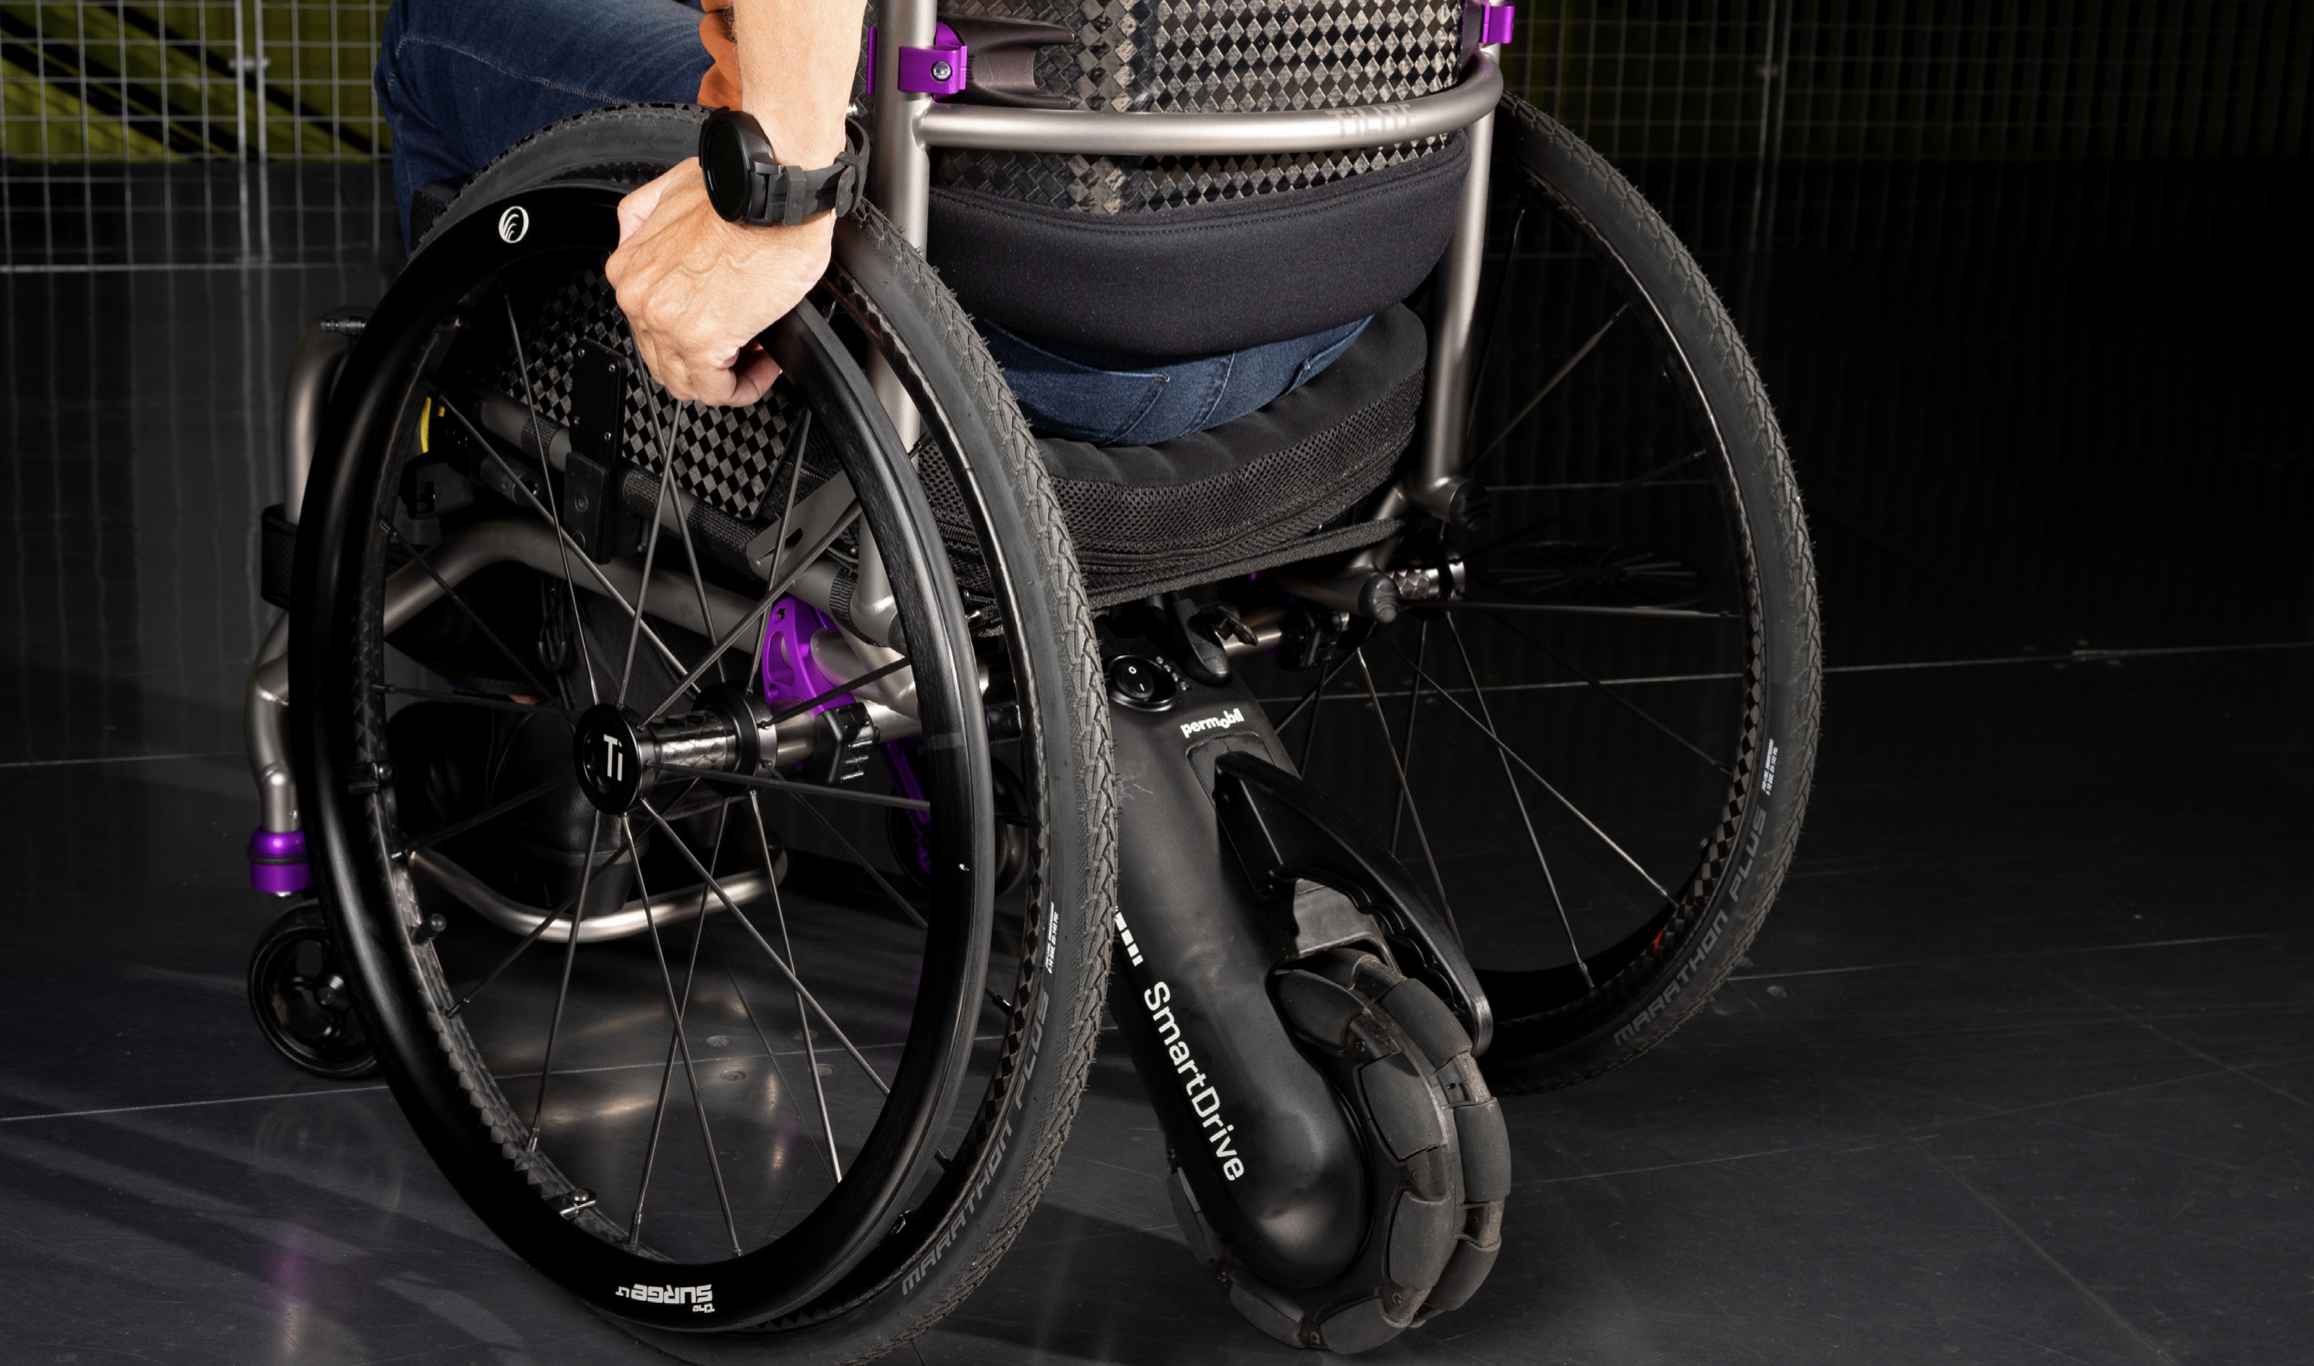
\includegraphics[height=50mm]{graphics/permobil.png}
    \caption{Permobil Smartdrive MX2+ Power Add-On Kit \cite{permobil_smartdrive_2022}.}
    \label{fig:permobil}
\end{figure}

It uses a 250W brushless dc motor to power the chair, giving it a maximum speed of 8.8 km/h and weighing only 5.7 kg for a user weight ranging from 14 to 150 kg.
Figure \ref{fig:permobil} shows the Permobil attached to a wheelchair. 
The user can turn the power assist on by using a wristband, PushTracker E2. 
The user can also change the speed settings and review system usage in the PushTracker E2. 
Permobil comes with a Switch Control, that can be adjusted to the user, which can provide momentary burst of power or  consistent power over extended distances \cite{permobil_smartdrive_2022}. 


\subsection{Airwheel SR5}
The Airwheel SR5 is a smart following suitcase. 
It uses UWB high-accuracy location technology to track the smart band the user has on, recognizing the distance between the user and suitcase.
It has two modes; auto-follow mode, and normal tow mode. 
If the suitcase is in auto-follow mode, it will draw up the motor, using 20W motor, to protect it and make it easy for the user to tow the luggage.
The SR5 has bluetooth 4.0, so it can be connected to the users smartphone, making it easy for the user to change settings like changing speed and to drive the suitcase manually. 
To detect obstacles it uses ultrasonic infrared sensor and plans dynamically to avoid them. 
It can reach up to 6 km/h with two 50 W motors, rated at speed 500 rpm. 
The SR5 is powered by a lithium-ion battery which weighs 340g and battery capacity of 62.6Wh.
The total weight of the suitcase is 6kg. 
The Airwheel SR5 can be seen in figure \ref{fig:airwheelsr5} along with the smart band \cite{airwheel_functions_2022}. 

\begin{figure}[!ht]
    \centering
    \includegraphics[height=50mm]{graphics/airwheel_sr5.png}
    \caption{Airwheel SR5 along with the Smart Band \cite{airwheel_functions_2022}.}
    \label{fig:airwheelsr5}
\end{figure}



\subsection{Robotic Wheelchair with Omni-directional vision}
This wheelchair was a project done at Saitama University and can the overview of the chair be seen in figure \ref{fig:omni-chair}. 
The robotic wheelchair was developed so that it could move alongside the users companion by observing his/her behavior such as body position and orientation.

\begin{figure}[!ht]
    \centering
    \includegraphics[height=60mm]{graphics/omni-vision wheelchair.png}
    \caption{Robotic Wheelchair with Omni-directional vision \cite{kobayashi_robotic_2012}.}
    \label{fig:omni-chair}
\end{figure}

The companion sets his/her initial position by tapping his/her facial image which is provided by the omni-directional camera.
The wheelchair has a laser range sensor, UTM-30LX by Hokuyo Electric Machinery, attached to a pole which is affixed to the wheelchair to be able to observe the upper body of the companion.
To observe the environment around itself it has 3 additional laser range sensors, URG-04LX. 
The wheelchair has an extension unit attached too the joystick controller to override the output signal generated by the software.
The lever of the joystick controller has been replaced with a touch-sensitive one so when the user touches the lever the control commands of the user override the signals from the software to ensure the safety of the user.

The wheelchair has three modes; side-following mode where the wheelchair is by the side of the companion, back-following mode where the wheelchair is behind the companion and insensitive mode where the wheelchair stops because the companion has stopped. 
The wheelchair desires to be in the side-following mode, but when the wheelchair senses that it can not be by its companion's side, it switches to the back-following mode until it is secure to return to the companion's side. 
The insensitive mode it entered when the chair senses that the companion has been stopped for 5 seconds and does not leave this mode until the companion is more than 80cm away from the wheelchair.
When leaving the insensitive mode the wheelchair goes to the back-following mode.
If the wheelchair loses his companion the system on the wheelchair can promptly re-identify the companion by using color appearances cues \cite{kobayashi_robotic_2012}.


\subsection{The Model H Hybrid}
Model H Hybrid as seen in figure \ref{fig:ModlHHybrid} is a true hybrid chair meaning that it can both be self-propelled by the user or use power to drive the motors so it can propel itself at any time.

\begin{figure}[!ht]
    \centering
    \includegraphics[height=55mm]{graphics/Hybrid_stóll.png}
    \caption{Model H Hybrid - The Hybrid Wheelchair \cite{jdy_imports_model_2022}.}
    \label{fig:ModlHHybrid}
\end{figure}

The chair is equipped with removable seat and seat belts, basic anti-tippers to prevent tipping forward or backwards, advanced lithium-ion batteries, a charger and 2 powerful motors to propel the wheelchair forwards or backwards should the user demand it. 
The batteries are 24V 6Ah lithium ion batteries. They give the wheelchair a range up to 8 miles or almost 13 km and a max speed of 5 mph or 8 km/h.
The chair itself is incredibly light or 39 lbs (17.7 kg) and can handle a maximum weight up to 240 lbs, roughly 109 kilos. 
It also comes with a joystick to control and move it around. The key feature in this specific design is that it is incredibly light, as talked about before, compering to other electric wheelchairs and they are proud to be the lightest mobility chairs on the planet.
They are also easily foldable and can fit into almost all vehicles which gives them a great competitive edge.
What this design lacks is the ability to follow its user should the user decide to stand up and walk a short distance given that the user is not fully paralyzed \cite{jdy_imports_model_2022}.


\subsection{Person following robot CNN}
This is a project that was done at York University, Toronto Canada, where students integrated stereo vision with a CNN Tracker for a person-following robot. The tracker is able to track a human in real time using an online convolutional neural network. The robot is able to follow the target around corners even when it is momentarily unseen by estimating and replicating the local path of the target.
The person following robot can be seen in Figure \ref{fig:follow-robot}

\begin{figure}[!ht]
    \centering
    \includegraphics[height=60mm]{graphics/preson-following-robot.png}
    \caption{A person following robot with stereo vision based CNN tracker\cite{raghavender_sahdev_person_2017}.}
    \label{fig:follow-robot}
\end{figure}

The robot used is a Pioneer 3-AT robot, which is a small four-wheel, four-motor skid-steer robot ideal for all-terrain operation or laboratory experimentation. The Pioneer 3-AT comes complete with one battery, emergency stop switch, wheel encoders and a microcontroller with ARCOS firmware, as well as Pioneer SDK advanced mobile robotics software development package. 
The students equipped and tested this robot with two stereo cameras, the Point Grey Bumblebee2 from Teledyne Flir and the ZED stereo camera from Stereolabs, which act as the only sensors on the robot to sense its environment.
An online convolutional neural network (CNN) is used to track the given target under different situations, making use of RGB images and a stereo depth image for tracking, as well as a novel stereo dataset. A PID based controller is then used to steer in such a way so as to keep the target in the center of the image.
Possible future work includes incorporating dynamic obstacle avoidance
techniques with the person following robot to give it more intelligence.

\section{Performance Metrics}

Customer needs were developed from interviewing the stakeholders, and the previous study, made by our stakeholder, Jón. 
The customer needs were organized by grouping together similar needs. 
Then the needs were organized into an hierarchy, which can be seen in table \ref{tab:customerneeds}. 
Latent needs were also identified and can also been seen in table \ref{tab:customerneeds}, denoted by !.
A list of metrics was prepared, and competitive benchmarking information was collected. 
The competitive benchmarking chart can be seen in table \ref{tab:metric}. 
The competitive benchmarking chart was then converted to table \ref{tab:bench_markt}, which considers perceived satisfaction of needs.
 

% listað upp 
\begin{table}[!ht]
\centering
\label{tab:customerneeds}
\caption{Customer needs and their importance. Importance ratings are indicated by the number of *'s, with *** denoting critically important needs. Latent needs are denoted by !.}
\scalebox{0.87}
{\begin{tabular}{clclll}
\hline
\multicolumn{1}{l}{\textbf{No.}} & \multicolumn{1}{c}{\textbf{Customer Needs}}                                                                               & \multicolumn{1}{l}{\textbf{Importance}} \\ \hline \hline
\textbf{1}           & \textbf{The wheelchair can move remotely}        & \textbf{***} \\
1.1                  & The wheelchair can accelerate                    & \textbf{***} \\
1.2                  & The wheelchair can turn                           & \textbf{**} \\ \\
\textbf{2}           & \textbf{The wheelchair is safe}                   &    \textbf{***}  \\
2.1                  & The wheelchair senses accurately / is reliable    & \textbf{***}  \\
2.2                  & The   wheelchair can be aware of its surrounding    & \textbf{**}  \\
2.3     & The   wheelchair doesn‘t bump into the user     & \textbf{***}   \\
2.4                  & The wheelchair can handle obstacles       & \textbf{**}  \\
2.5                  & The wheelchair can follow the user through doors   & \textbf{*}\\
2.6                  & The wheelchair can know where the user is & \textbf{***}  \\ \\
\textbf{3}           & \textbf{The wheelchair is practical}       & \textbf{***}  \\
3.1                  & The wheelchair cannot be heavy   & \textbf{***}               \\
3.2                  & The wheelchair hardware can be easily affixed   & \textbf{**}      \\
3.3                  & \begin{tabular}[c]{@{}l@{}}Can work as a standard wheelchair when\\ feature is not on\end{tabular}   & \textbf{***}    \\
\multicolumn{1}{l}{3.4} & The wheelchair is not loud   & \textbf{!}   \\ \\
\textbf{4}           & \textbf{The wheelchair is durable}   & \textbf{**} \\
4.1                  & The wheelchair can handle an hour session at a time  & \textbf{**}  \\ \\
\textbf{5}           & \textbf{The wheelchair provides feedback}       &    \textbf{**}                     \\
5.1                  & \begin{tabular}[c]{@{}l@{}}The wheelchair lets the user know if something is wrong, \\ i.e. far behind/stuck\end{tabular} & \textbf{***}  \\
5.2   & The wheelchair can communicate with the user   & \textbf{**}   \\
5.3 & The wheelchair can let the user know the distance he walked & \textbf{!}  \\ \hline
\end{tabular}}
\end{table}



%Competitive benchmarking chart based on metrics

\begin{table}[h]
\caption{Competitive benchmarking chart based on metrics. * denotes an educated guess based on information provided by the source of the product/project. N/A is used for not applicable and N/S is used for not specified.}
\resizebox{\textwidth}{!}{\begin{tabular}{|c|c|c|c|c|c|c|c|c|c|}
\hline
\begin{tabular}[c]{@{}c@{}}No.\end{tabular} & \begin{tabular}[c]{@{}c@{}}Need \\ No.\end{tabular}     & Metric                                                                                                 & Imp & Unit   & \begin{tabular}[c]{@{}c@{}}Permobil \\ Smartdrive \\ MX2+\\Power \\ Add-On Kit\end{tabular} & \begin{tabular}[c]{@{}c@{}}Airwheel \\ SR5\end{tabular} & \begin{tabular}[c]{@{}c@{}}Robotic\\Wheelchair \\ with \\ Omni-
\\directional \\ vision\end{tabular} & \begin{tabular}[c]{@{}c@{}}The Model \\ H Hybrid\end{tabular} & \begin{tabular}[c]{@{}c@{}}Person \\ following \\ Robot \\CNN\end{tabular} \\ \hline
1 & 1, 2.3  & \begin{tabular}[c]{@{}c@{}}Distance\\from user\end{tabular}  & 5   & m & N/A  & N/S  & N/S  & N/A   & 1     \\ \hline
2   & 1.1   & Speed    & 5   & km/h   & 8.8  & 6 & N/S  & 8   & 3.6      \\ \hline
3  & 1.2   & Rotation & 5   & deg    & N/A  & 360* & 360* & 360*  & 360*  \\ \hline
4  & 2 & VOTTUN!!!!!! & 4   & binary & Pass   & N/A  & Fail*    & Pass*    & Fail   \\ \hline
5    & 2.1  & \begin{tabular}[c]{@{}c@{}}Sensor have small\\ margin of error\end{tabular}& 4   & \%     &  N/S  & Low*  & Low*   & N/A  & Low*   \\ \hline
6  & 2.2   & \begin{tabular}[c]{@{}c@{}}Reacts to\\environment \end{tabular}  & 4   & s  & N/A   & 1*   & 3*  & N/A   & 2*       \\ \hline
7 & 2.4 & \begin{tabular}[c]{@{}c@{}}Minimum\\distance\\  from obstacles\end{tabular} & 4  & m  &  N/A &  N/S & N/S  & N/A &  N/S\\ \hline
8  & 2.5  & Door test  & 1   & binary & Pass & Pass    & Pass    & Pass     & Pass   \\ \hline
9  & 2.6     & \begin{tabular}[c]{@{}c@{}}Coordinates\\ comparing from \\ user device to \\ the wheelchair\end{tabular} & 5 & deg    & N/A &  N/S   & N/A  & N/A & N/A   \\ \hline
10 & 3  & \begin{tabular}[c]{@{}c@{}}How likely is \\ the user to \\ use the product\end{tabular}  & 4   & subj.  & ?????             & ????  & ?????   & ?????  & ?????  \\ \hline
11 & 3.1 & Total mass of kit & 4   & kg     & 5.7   & 6  & N/S   & 17.7   & 15* 
\\ \hline
12 & 3.2      & \begin{tabular}[c]{@{}c@{}}Time to assemble \\ for the first \\time\end{tabular}  & 2   & s      & 60*     & 0*   & 0*  & 0*    &  N/S \\ \hline
13 & 3.2   & \begin{tabular}[c]{@{}c@{}}80\% of user can\\  assemble without \\ assistance\end{tabular}  & 1   & binary &  N/S    & Pass*  & Pass*    & Pass* &  N/S  \\ \hline
14     & 3.3   & \begin{tabular}[c]{@{}c@{}}Manual propelling \\ available\end{tabular}   & 5   & binary & Pass   & Pass & Fail & Pass & N/A     \\ \hline
15 & 3.4  & Maximum noise  & 2   & dB     &  N/S    & Mute &  N/S  &  N/S &  N/S     \\ \hline
16  & 4       & \begin{tabular}[c]{@{}c@{}}Durability longer \\ than 3 years\end{tabular} & 3   & years  & 2+  &  N/S&  N/S  & 5+   &  N/S  
\\ \hline
17 & 4.1  & \begin{tabular}[c]{@{}c@{}}Minimum\\duration\end{tabular}  & 3  & km  & 19.8 & 5  &  N/S  & 13  &  N/S 
\\ \hline
18   & 5   & \begin{tabular}[c]{@{}c@{}}Conveys messages\\  to user\end{tabular}   & 4   & binary & Pass  & Pass & Fail  & Fail  & Pass                              \\ \hline
19 & \begin{tabular}[c]{@{}c@{}}5.1,\\ 5.2,\\ 5.3\end{tabular} & \begin{tabular}[c]{@{}c@{}}Minimum volume\\from message\end{tabular}& 3   & dB     &  N/S  &  N/S   &  N/S  & N/A  &  N/S \\ \hline
20 & 5.1 &\begin{tabular}[c]{@{}c@{}} Minimum \\vibration \end{tabular} & 1 & Hz &  N/S  &  N/S & N/A & N/A & N/A  \\ \hline
21 & 5.2 & \begin{tabular}[c]{@{}c@{}}Minimum\\ luminance\\ of LED\end{tabular} & 2 & Lumens &  N/S &  N/S & N/A &  N/S &  N/S \\ \hline
22 & 5.3 & \begin{tabular}[c]{@{}c@{}}Keep track\\of distance \end{tabular}  & 1   & binary & Pass   & 170-240*   &  N/S  & N/A& N/A \\ \hline
23 & 5.3 & Screen message & 1   & binary & Pass  & Pass  & Fail & Fail & N/A \\ \hline
\end{tabular}}
\label{tab:metric}
\end{table}


% Competitive benchmarking chart based on perceived satisfaction of needs.
\begin{table}[h]
\caption{Competitive benchmarking chart based on perceived satisfaction of needs. (Scoring more “dots” corresponds to greater perceived satisfaction of the need.)}
\resizebox{\textwidth}{!}{\begin{tabular}{|c|c|c|c|c|c|c|c|}
\hline
\textbf{No.} & \textbf{Need} & \textbf{Imp} & \textbf{\begin{tabular}[c]{@{}c@{}}Permobil \\ Smartdrive \\ MX2\end{tabular}} & \textbf{\begin{tabular}[c]{@{}c@{}}Airwheel \\ SR5\end{tabular}} & \textbf{\begin{tabular}[c]{@{}c@{}}Robotic \\ Wheelchair\end{tabular}} & \textbf{\begin{tabular}[c]{@{}c@{}}Model\\H \\ Hybrid\end{tabular}} & \textbf{\begin{tabular}[c]{@{}c@{}}Person \\Following \\ Robot\end{tabular}} \\ \hline
1. & \textbf{\begin{tabular}[c]{@{}c@{}}Can move \\ remotely\end{tabular}} & 5 & * & ***** & ***** & * & ***** \\ \hline
1.1 & Can move & 5 & ****** & ***** & ***** & ***** & ***** \\ \hline
1.2 & Can turn & 4 & *** & ***** & ***** & ***** & ***** \\ \hline
2 & \textbf{Is safe} & 5 & ** & ***** & **** & ***** & *** \\ \hline
2.1 & \begin{tabular}[c]{@{}c@{}}Senses accurately \\ /is reliable\end{tabular} & 4 & * & ***** & ***** & * & ***** \\ \hline
2.2 & \begin{tabular}[c]{@{}c@{}}Is aware of \\ its surroundings\end{tabular} & 3 & * & ***** & ***** & * & ***** \\ \hline
2.3 & \begin{tabular}[c]{@{}c@{}}Doesn‘t bump \\ into the user\end{tabular} & 5 & * & ***** & ***** & * & **** \\ \hline
2.4 & \begin{tabular}[c]{@{}c@{}}Can handle \\ obstacles\end{tabular} & 4 & * & ***** & ***** & * & * \\ \hline
2.5 & \begin{tabular}[c]{@{}c@{}}Can follow the \\ user through doors\end{tabular} & 2 & * & ***** & ***** & * & **** \\ \hline
2.6 & \begin{tabular}[c]{@{}c@{}}Can know where\\  the user is\end{tabular} & 5 & * & ***** & ***** & * & ***** \\ \hline
3 & \textbf{Is practical} & 4 & **** & **** & *** & ** & *** \\ \hline
3.1 & Can not be heavy & 5 & ***** & **** & * & ***** & **** \\ \hline
3.2 & \begin{tabular}[c]{@{}c@{}}Hardware can\\  be easily affixed\end{tabular} & 3 & **** & **** & *** & ***** & *** \\ \hline
3.3 & \begin{tabular}[c]{@{}c@{}}Can work as a \\ standard wheelchair \\ when feature\\is not on\end{tabular} & 5 & ***** & * & * & ***** & * \\ \hline
3.4 & Is not loud & 2 & *** & *** & **** & *** & *** \\ \hline
4 & \textbf{Is durable} & 2 & ***** & ** & ***** & ***** & ** \\ \hline
4.1 & \begin{tabular}[c]{@{}c@{}}Can handle an \\ hour session\\at a time\end{tabular} & 3 & ***** & **** & ***** & ***** & *** \\ \hline
5 & \textbf{Provides feedback} & 4 & *** & ***** & *** & * & **** \\ \hline
5.1 & \begin{tabular}[c]{@{}c@{}}Lets the user\\  know if something \\ is wrong,\\  i.e. far behind/stuck\end{tabular} & 4 & * & ***** & * & * & ** \\ \hline
5.2 & \begin{tabular}[c]{@{}c@{}}Can communicate\\  with the user\end{tabular} & 4 & ** & ***** & *** & ** & ** \\ \hline
5.3 & \begin{tabular}[c]{@{}c@{}}Can let the user \\ know the distance\\  he walked\end{tabular} & 1 & ***** & * & * & * & * \\ \hline
\end{tabular}}
\label{tab:bench_markt}
\end{table}
\chapter{Target Cost}
The value of the manufacturing cost specification based on the price our company hopes the end user will pay for the product and on the profit margins that are required for each stage in the distribution channel. The product is in the early stages of product-design so the cost analysis is only based on assumptions. Stuðlaberg sells the product Permobil and the cost of said product is 878.180 ISK. Simular product can be seen listed in table \ref{tab:cost_analysis}.

\begin{table}[!h]
    \centering
        \setlength{\tabcolsep}{18pt}
        \renewcommand{\arraystretch}{1.2}
        \begin{tabular}{ll}
\hline
Name & Cost [ISK] \\ 
\hline\hline
Airwheel SR5 & 123.445 \cite{airwheel_functions_2022}\\
Robotic Wheelchair & \\
Model H Hybrid & 304.817 \cite{jdy_imports_model_2022}\\
Person Following Robot & \\
\hline
\end{tabular}
\caption{Table that show the price of similar products.}
\label{tab:cost_analysis}
\end{table}

\bibliographystyle{IEEEtran/bibtex/ieeetran}
\bibliography{references}


%% If appendices are needed, uncomment the following line
%% and include the appendices in separate files
\appendix{}%%RUM: "Appendicies (as appropriate)
\chapter{Target Cost}
The value of the manufacturing cost specification based on the price our company hopes the end user will pay for the product and on the profit margins that are required for each stage in the distribution channel. The product is in the early stages of product-design so the cost analysis is only based on assumptions. Stuðlaberg sells the product Permobil and the cost of said product is 878.180 ISK. Simular product can be seen listed in table \ref{tab:cost_analysis}.

\begin{table}[!h]
    \centering
        \setlength{\tabcolsep}{18pt}
        \renewcommand{\arraystretch}{1.2}
        \begin{tabular}{ll}
\hline
Name & Cost [ISK] \\ 
\hline\hline
Airwheel SR5 & 123.445 \cite{airwheel_functions_2022}\\
Robotic Wheelchair & \\
Model H Hybrid & 304.817 \cite{jdy_imports_model_2022}\\
Person Following Robot & \\
\hline
\end{tabular}
\caption{Table that show the price of similar products.}
\label{tab:cost_analysis}
\end{table}

%\backmatter{} % Sections after this don't get numbers
%% We prefer that all elements be numbered

%%%%%%%%%%%%% SHOW INDEX %%%%%%%%%%%%%%%%%%
%% Index, optional.  A good idea on longer documents
\clearforchapter{}
\printindex{}%%RUM: Not mentioned

\end{document}
%%% Local Variables:
%%% mode: latex
%%% TeX-master: t
%%% TeX-engine: luatex
%%% End:
